\documentclass{beamer}

\mode<presentation> {
%  \usetheme{Warsaw}
	\usetheme{Boadilla}
	\setbeamercovered{transparent}
}

%\usepackage{ucs}
\usepackage[utf8]{inputenc}
\usepackage[czech]{babel}
%\usepackage{palatino}
\usepackage{graphicx}
\usepackage{listings}

\title[Bitlocker šifrování v Linuxovém prostředí]{Bitlocker šifrování v Linuxovém prostředí\\\small{Diplomová práce -- kontrolní den č. 2}}
\author{Vojtěch Trefný}
\institute[FAI UTB]{Fakulta aplikované informatiky UTB}
\date{5.~4.~2019}

\begin{document}

\begin{frame}
	\titlepage
\end{frame}

\begin{frame}
	\frametitle{Osnova}
	\tableofcontents
\end{frame}

%%%%%%%%%%%%%%%%%%%%%%%%%%%%%%%%%%%%%%%%%%%%%%%%%%%%%%%%%%%%%%%%%%

\section{Zadání}

\begin{frame}
	\frametitle{Zadání}
	\begin{block}{}
		\begin{itemize}
			\item \textbf{Vedoucí:} Ing. Michal Bližňák Ph.D.
			\item \textbf{Konzultant:} Ing. Milan Brož Ph.D. (Red Hat Czech/CRoCS FI MUNI)
		\end{itemize}
	\end{block}

	\begin{block}{}
		\begin{itemize}
			\item Seznamte se s nástrojem Windows Bitlocker pro šifrování disků.
			\item Popište podporované šifrovací módy a možnosti správy klíčů.
			\item Analyzujte použitá kryptografická primitiva a jejich atributy.
			\item Seznamte se s nástrojem a knihovnou libbde a možnostmi přístupu k Bitlocker obrazu disku v prostředí OS Linux.
			\item Navrhněte a podle možností implementujte nutná rozšíření Linuxových nástrojů pro jednoduchý přístup k obsahu Bitlocker disku.
		\end{itemize}
	\end{block}

\end{frame}

%%%%%%%%%%%%%%%%%%%%%%%%%%%%%%%%%%%%%%%%%%%%%%%%%%%%%%%%%%%%%%%%%%

\section{Postup implementace}

\begin{frame}
	\frametitle{Implementace}
	\begin{block}{Získání (de)šifrovacího klíče}
		\begin{itemize}
			\item Vlastní jednoduchý program, který z BitLocker hlaviček (při znalosti hesla) získá klíč pro (de)šifrování dat (FVEK).
			\item Klíč samotný je uložený v metadatové části zařízení zašifrovaný dalším klíčem (VMK), který je zašifrován klíčem odvozeným z hesla.
		\end{itemize}
	\end{block}

	\begin{block}{Identifikace datových oblastí}
		\begin{itemize}
			\item Vlastní zašifrovaná dat jsou na disku uložena nesouvisle, prokládaná metadaty.
			\item Prvních 16 sektorů (NTFS hlavička) je uloženo na speciálním offsetu.
		\end{itemize}
	\end{block}
\end{frame}

\begin{frame}
	\frametitle{Implementace II}

	\begin{block}{Device mapper}
		\begin{itemize}
			\item Za znalosti (de)šifrovacího klíče a struktury dat na disku lze vytvořit device-mapper zařízení.
			\item Data jsou (de)šifrována dle potřeby v době čtení/zápisu daného sektoru.
		\end{itemize}
	\end{block}

\begin{figure}[ht!]
	\begin{center}
  	  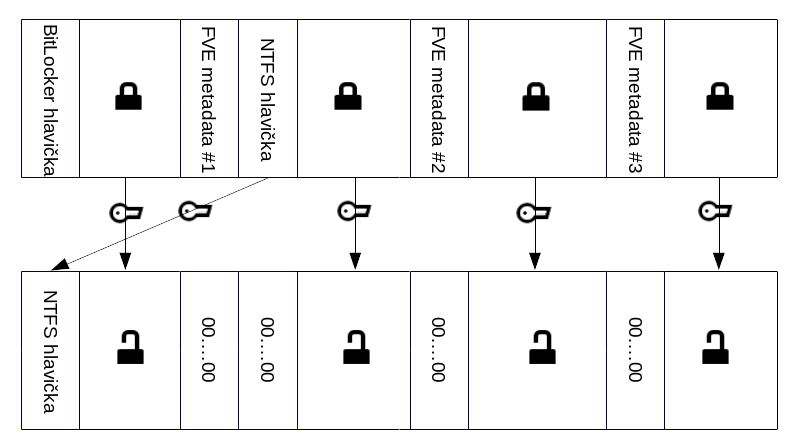
\includegraphics[width=9cm]{img/bitlocker-decrypt-schema.png}
	\end{center}
	\end{figure}


\end{frame}

\begin{frame}[fragile]
	\begin{lstlisting}[frame=none, basicstyle=\ttfamily\small, columns=fullflexible, keepspaces=true]
$ sudo bitlockersetup /dev/sdc2 bitlocker
Password for '/dev/sdc2': 
Created device mapper device '/dev/mapper/bitlocker'.

$ lsblk -f /dev/sdc2
NAME        FSTYPE LABEL UUID
sdc2                                                          
\_bitlocker ntfs         A4843D7D843D5352

$ sudo dmsetup table --showkeys bitlocker
0 16 crypt aes-xts-plain64 a4d0...f52 68904 8:34 68904
16 68760 crypt aes-xts-plain64 a4d0...f52 16 8:34 16
68776 128 zero 
68904 16 zero 
68920 21424 crypt aes-xts-plain64 a4d0...f52 68920 8:34 68920
90344 128 zero 
90472 22632 crypt aes-xts-plain64 a4d0...f52 90472 8:34 90472
113104 128 zero 
113232 91568 crypt aes-xts-plain64 a4d0...f52 113232 8:34 113232
	\end{lstlisting}

\end{frame}

%%%%%%%%%%%%%%%%%%%%%%%%%%%%%%%%%%%%%%%%%%%%%%%%%%%%%%%%%%%%%%%%%%

\section{Další kroky}

\begin{frame}
  \frametitle{Další kroky}
	\begin{block}{}
		\begin{itemize}
			\item Rozsáhlejší testování -- integrita dat a souborového systému po zápisu, extrémně velká zařízení, zaplnění zařízení...
			\item Integrace s nástroji pro správu blokových zařízení v Linuxu:
			\begin{itemize}
				\item UDev, libblkid -- detekce BitLocker signatury
				\item libblockdev -- API pro odemykání
				\item UDisks -- detekce, DBus API pro odemykání (pro GVFS)
			\end{itemize}
			\item Doladění existující implementace -- chybové stavy, záložní heslo...
			\item Podpora ostatních (starších a méně obvyklých) variant BitLockeru.
			\item Práce na textové části práce.
		\end{itemize}
	\end{block}

\end{frame}

%%%%%%%%%%%%%%%%%%%%%%%%%%%%%%%%%%%%%%%%%%%%%%%%%%%%%%%%%%%%%%%%%%

\section{Postup splnění zadání}

\begin{frame}
  \frametitle{Procentuální splnění zadání}
	\begin{block}{Rešerše}
		\begin{itemize}
			\item seznámení s nástrojem BitLocker -- \textbf{100 \%}
			\item seznámení s existujícími řešeními (libbde, dislocker) -- \textbf{100 \%}
			\item popis šifrovacích módů, správy klíčů, použitých kryptografických fcí -- \textbf{15 \%}
		\end{itemize}
	\end{block}

	\begin{block}{Implementace}
		\begin{itemize}
			\item nástroj pro práci s BitLocker v Linuxu -- \textbf{90 \%}
			\item integrace s existujícími nástroji pro práci se storage -- \textbf{20 \%}
		\end{itemize}
	\end{block}

\end{frame}

%%%%%%%%%%%%%%%%%%%%%%%%%%%%%%%%%%%%%%%%%%%%%%%%%%%%%%%%%%%%%%%%%%

\section{Závěr}

\begin{frame}
	\frametitle{Závěr}

	\begin{center}
	Děkuji vám za pozornost.
	\end{center}

\vspace{0.5cm}

	\begin{center}
	Prostor pro vaše dotazy.
	\end{center}
\end{frame}

\end{document}
